\question

\ifspanish
Considere un problema de detección con tres hipótesis ($H \in\{0,1,2\}$) y observación $\mathbf{X} = (X_1, X_2)^T \in \mathbb{R}^2$. Asimismo, se sabe que las hipótesis son equiprobables y que
\else
Consider a detection problem with three hypothesis ($H \in\{0,1,2\}$) and observation $\mathbf{X} = (X_1, X_2)^T \in \mathbb{R}^2$. Moreover, we know that hypotheses are equally likely, also that
\fi
\begin{equation*}
p_{X_1|X_2,H}(x_1|x_2,0) = p_{X_1|X_2,H}(x_1|x_2,1) = p_{X_1|X_2,H}(x_1|x_2,2),
\end{equation*}
\ifspanish y \else and \fi
\begin{align*}
  p_{X_2|H}(x_2|0) &= \begin{cases} 1/3, & |x_2| < 1.5, \\ 0, & \text{otherwise}, \end{cases} \\
  p_{X_2|H}(x_2|1) &= \begin{cases} x_2/2, & 0 < x_2 < 2, \\ 0, & \text{otherwise}, \end{cases}\\
  p_{X_2|H}(x_2|2) &= \begin{cases} -x_2/2, & -2 < x_2 < 0, \\ 0, & \text{otherwise}. \end{cases}
\end{align*}

\ifspanish Determine las regiones de decisión del detector que minimiza la probabilidad de error
\else Derive the decision regions of the detector that minimizes the probability of error.
\fi

\begin{solution}
\ifspanish El detector que minimiza la probabilidad de error es el detector MAP, dado por
\else The detector that minimizes the probability of error is the MAP detector, which is given by
\fi
\begin{equation*}
d = \arg \mathop{\operatorname{max}}_{h} P_{H|\mathbf{X}}(h|\mathbf{x}),
\end{equation*}
\ifspanish y puede reescribirse como \else and can be rewritten as \fi
\begin{equation*}
d = \arg \mathop{\operatorname{max}}_{h} p_{\mathbf{X}|H}(\mathbf{x}|h) P_H(h) 
  = \arg \mathop{\operatorname{max}}_{h} p_{\mathbf{X}|H}(\mathbf{x}|h),
\end{equation*}
\ifspanish donde el último paso se sigue de $P_H(h) = 1/M$. Sin embargo, no se tiene la verosimilitud conjunta $p_{\mathbf{X}|H}(\mathbf{x}|h)$, sino solamente $p_{X_1|X_2,H}(x_1|x_2,h)$ y $p_{X_2|H}(x_2|h)$. Aplicando el teorema de Bayes, la verosimilitud conjunta resulta
\else where the last step follows from $P_H(h) = 1/M$. However, we do not have the joint likelihood $p_{\mathbf{X}|H}(\mathbf{x}|h)$, but only $p_{X_1|X_2,H}(x_1|x_2,h)$ and $p_{X_2|H}(x_2|h)$. Using Bayes's theorem, the joint likelihood becomes
\fi
\begin{equation*}
p_{\mathbf{X}|H}(\mathbf{x}|h) = p_{X_1,X_2|H}(x_1,x_2|h) = p_{X_1|X_2,H}(x_1|x_2,h) p_{X_2|H}(x_2|h),
\end{equation*}
\ifspanish que conduce a \else which yields \fi
\begin{align*}
d &= \arg \mathop{\operatorname{max}}_{h} p_{\mathbf{X}|H}(\mathbf{x}|h) 
   = \arg \mathop{\operatorname{max}}_{h} p_{X_1|X_2,H}(x_1|x_2,h) p_{X_2|H}(x_2|h) \\ 
  &= \arg \mathop{\operatorname{max}}_{h} p_{X_2|H}(x_2|h),
\end{align*}
\ifspanish donde, en el último paso, se ha tenido en cuenta que $p_{X_1|X_2,H}(x_1|x_2,h)$ no depende de $h$. Por tanto, las regiones de decisión solamente pueden depender de $x_2$ y, para determinarlas, se necesita $p_{X_2|H}(x_2|h)$, que se muestra en la figura siguiente
\else where, in the last step, we have taken into account that $p_{X_1|X_2,H}(x_1|x_2,h)$ does not depend on $h$. Then, the decision regions can only depend on $x_2$ and, to derive them, we need $p_{X_2|H}(x_2|h)$, which is plotted in the following figure
\begin{center}
		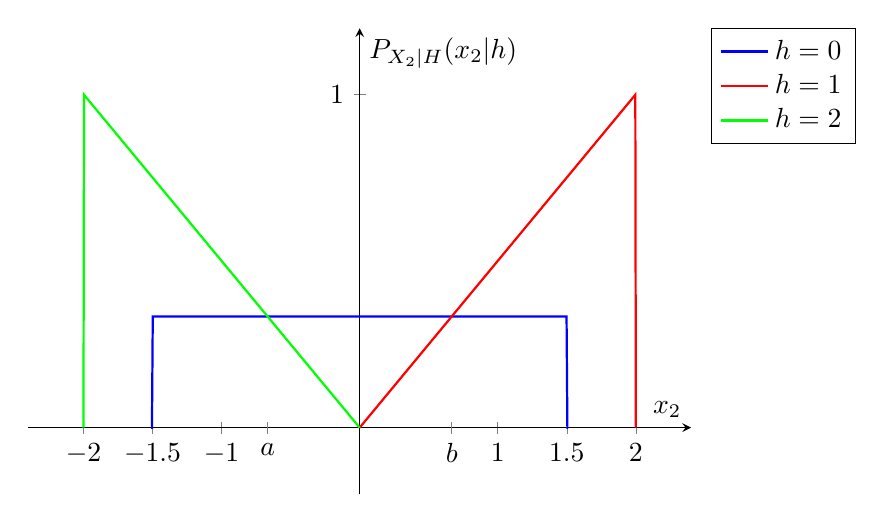
\begin{tikzpicture}
		\begin{axis}[%
		axis x line=middle,
		axis y line=middle,
		enlarge x limits=0.1,
		enlarge y limits=0.2,
		xtick={-2,-1.5,-1,0,1,1.5,2},
		%xticklabels={$-\pi$,$-\frac{2\pi}{N}$,$\frac{2\pi}{N}$,$\pi$},
		extra x ticks={-2/3,2/3},
		extra x tick labels={$a$,$b$},
		xmin=-2,
		xmax=2,
		ymin=0,
		%ytick=\empty,
		ytick={0,1},
		width=10cm,
		height=7.5cm,
		domain = -2:2,
		samples = 512,
		xlabel={$x_2$},
		ylabel={$P_{X_2|H}(x_2|h)$},
		legend pos=outer north east]
		\addplot[blue,thick,domain=-1.51:1.51] {1/3*(abs(x)<1.5)};
		\addlegendentry{$h = 0$};
		\addplot[red,thick,domain=0:2] {x/2*(x>0 && x<2)};
		\addlegendentry{$h = 1$};
		\addplot[green,thick,domain=-2:0] {-x/2*(x<0 && x>-2)};
		\addlegendentry{$h = 2$};
		\end{axis}
		\end{tikzpicture}
	\end{center}

\ifspanis Por tanto, las regiones de decisión, que están definidas por \else Hence, the decision regions, which are defined as \fi
  \begin{equation*}
    \mathcal{X}_d = \{\mathbf{x} | d = \arg \mathop{\operatorname{max}}_{h} p_{X_2|H}(x_2|h)\},
  \end{equation*}
\ifspanish están dadas por \else are given by \fi
\begin{align*}
\mathcal{X}_0 &= \{x_2 \in \mathbb{R}  \mid a < x_2 < b \},  \\
\mathcal{X}_1 &= \{x_2 \in \mathbb{R}  \mid b \leq x_2 < 2 \},
\mathcal{X}_2 &= \{x_2 \in \mathbb{R}  \mid -2 < x_2 \leq a \}.
\end{align*}
\ifspanish Por tanto, solamente resta determinar las fronteras de decisión, que son la solución de
\else Hence, it remains to find the decision boundaries, which are the solution to \fi
\begin{align*}
P_{X_2|H}(b|0) &= P_{X_2|H}(b|1) \Rightarrow b = \frac{2}{3},  \\
P_{X_2|H}(a|0) &= P_{X_2|H}(a|2) \Rightarrow a = -\frac{2}{3},
\end{align*}
\ifspanish resultando \else yielding \fi
\begin{align*}
\mathcal{X}_0 &= \{x_2  \in \mathbb{R} \mid -2/3 < x_2 < 2/3 \}, \\
\mathcal{X}_1 &= \{x_2  \in \mathbb{R} \mid 2/3 \leq x_2 < 2 \}, \\
\mathcal{X}_2 &= \{x_2  \in \mathbb{R} \mid -2 < x_2 \leq -2/3 \}.
\end{align*}
        
\end{solution}



